\documentclass[11pt,a4paper]{article}
\usepackage[utf8]{inputenc}
\usepackage[margin=1in]{geometry}
\usepackage{amsmath, amssymb, amsthm}
\usepackage{graphicx}
\usepackage{booktabs}
\usepackage{hyperref}
\usepackage{algorithm2e}
\usepackage{color}

\title{Advanced Job Sequencing with Deadlines:\\Algorithmic Optimizations, Extensions to Johnson's Rule, and xAI Integration}
\author{Musa \and Ha \and Justin \\ \medskip Yuan Ze University \\ \textit{Introduction to Algorithms - 114-2}}
\date{May 25, 2026}

\begin{document}

\maketitle

\begin{abstract}
This report provides a comprehensive study of the Job Sequencing with Deadlines problem, a classic single-machine scheduling optimization problem. We investigate three standard baseline algorithms: a Naive Greedy approach ($O(N^2)$), a Min-Heap optimized approach ($O(N \log N)$), and a Disjoint Set Union (DSU) optimized approach ($O(N \log D)$). Furthermore, we propose an ultra-efficient optimization that combines a linear-time Radix Sort with DSU, achieving $O(N \alpha(D))$ time complexity, which runs in practically linear time. We present empirical results on datasets ranging up to $N = 50,000$ jobs, showing that our proposed method outperforms the best baselines by up to 4x. Finally, we connect our work to the 2-machine flow shop problem solved by Johnson's Algorithm, and discuss the integration of Explainable AI (xAI) for deploying scheduling algorithms in real-world industrial environments.
\end{abstract}

\section{Introduction}
In industrial manufacturing, cloud computing, and logistics, scheduling jobs efficiently under time constraints is a fundamental problem. The \textbf{Job Sequencing with Deadlines} problem is defined as follows:
Given a set of $n$ jobs $S = \{J_1, J_2, \dots, J_n\}$, where each job $J_i$ has a deadline $d_i \ge 1$ and a profit $p_i \ge 0$. Each job takes exactly 1 unit of time to complete, and only one job can be processed at any given time. A job yields profit $p_i$ only if it is completed on or before its deadline $d_i$. The goal is to find a feasible schedule (a subset of jobs and an assignment of jobs to time slots) that maximizes the total profit.

\section{Mathematical Foundation: The Matroid Perspective}
The correctness of the greedy approach for Job Sequencing with Deadlines is mathematically justified by \textbf{Matroid Theory}.

A matroid is an ordered pair $M = (S, \mathcal{I})$ where $S$ is a finite set, and $\mathcal{I}$ is a family of subsets of $S$ (called independent sets) satisfying:
\begin{enumerate}
    \item \textbf{Hereditary Property:} If $A \in \mathcal{I}$ and $B \subseteq A$, then $B \in \mathcal{I}$.
    \item \textbf{Exchange Property:} If $A, B \in \mathcal{I}$ and $|A| < |B|$, there exists $x \in B \setminus A$ such that $A \cup \{x\} \in \mathcal{I}$.
\end{enumerate}

For Job Sequencing, we define a subset of jobs $I \subseteq S$ to be independent ($I \in \mathcal{I}$) if there exists a valid schedule for the jobs in $I$ such that no job violates its deadline.
\begin{theorem}
The pair $M = (S, \mathcal{I})$ defined above forms a matroid.
\end{theorem}
\begin{proof}
The hereditary property is trivial: if a set of jobs $A$ has a valid schedule, removing some jobs yields a subset $B \subseteq A$ which can also be scheduled legally by leaving the corresponding slots empty.
The exchange property can be proven by showing that if $|A| < |B|$, we can shift the scheduled times of jobs in $A$ to free up a slot for some job in $B \setminus A$.
By the Gale-Rado theorem, since $M$ is a matroid, a greedy algorithm that sorts elements by weight (profit) in descending order and greedily adds elements to the independent set is guaranteed to find a subset of maximum total profit.
\end{proof}

\section{Algorithmic Methods and Baselines}
We study three standard baselines from GeeksforGeeks and propose a fourth, highly-optimized algorithm:

\subsection{Naive Greedy Approach -- $O(N^2)$}
Sort all jobs in descending order of profit. For each job, scan backward from its deadline slot $\min(n, d_i) - 1$ down to 0 to find the first available free slot. If found, mark the slot as occupied and schedule the job. The worst-case complexity is $O(N^2)$ due to the nested loops.

\subsection{Min-Heap Optimized Approach -- $O(N \log N)$}
Sort all jobs in ascending order of their deadlines. Iterate through the sorted jobs and maintain a Min-Heap of the profits of scheduled jobs. For each job, if its deadline is greater than the size of the heap, push its profit to the heap. Otherwise, if its profit is greater than the top (minimum profit) of the heap, pop the top and push the new profit. This runs in $O(N \log N)$ time and $O(N)$ space.

\subsection{Disjoint Set Union (DSU) Approach -- $O(N \log D)$}
Sort all jobs in descending order of profit. Represent time slots $0 \dots D$ (where $D$ is the maximum deadline) as a disjoint set forest. The representative element of node $t$, found via \texttt{Find(t)}, points to the latest available slot $\le t$. When a slot is filled, we merge it with the slot immediately preceding it using \texttt{Union(Find(t)-1, Find(t))}. Dominating factor is sorting, making it $O(N \log N)$ overall, with slot finding taking $O(N \alpha(D))$.

\subsection{Proposed Optimization: Radix Sort + DSU -- $O(N \alpha(D))$}
The bottleneck in both the Heap and DSU approaches is the comparison-based sort ($O(N \log N)$). Since profits and deadlines are positive integers, we replace the standard sort with a stable \textbf{Radix Sort} (using base 256). For 32-bit integers, this requires exactly 4 passes, running in $O(N)$ time.
We then use DSU with path compression to find available slots in $O(N \alpha(D))$ time.
This reduces the entire scheduling algorithm to practically linear time, $O(N \alpha(D))$, bypassing the sorting bottleneck.

\section{Experimental Evaluation}
To evaluate these algorithms, we generated 6 random datasets ranging from $N = 10$ to $N = 50,000$ jobs. The results are summarized in Table~\ref{tab:benchmarks} and visualized in Figure~\ref{fig:comparison}.

\begin{table}[h]
\centering
\caption{Empirical execution times (in ms) of the scheduling algorithms.}
\label{tab:benchmarks}
\begin{tabular}{lcccc}
\toprule
\textbf{Jobs (N)} & \textbf{Naive $O(N^2)$} & \textbf{Min-Heap $O(N \log N)$} & \textbf{DSU $O(N \log D)$} & \textbf{Proposed Radix-DSU $O(N)$} \\
\midrule
10     & 0.0020 & 0.0030 & 0.0020 & 0.0030 \\
100    & 0.0140 & 0.0110 & 0.0130 & 0.0040 \\
500    & 0.0530 & 0.0630 & 0.0390 & 0.0220 \\
2,000  & 0.5710 & 0.2830 & 0.1980 & 0.0660 \\
10,000 & 13.8600 & 1.7930 & 1.1100 & 0.4380 \\
50,000 & Skipped & 8.7770 & 5.7520 & 2.3410 \\
\bottomrule
\end{tabular}
\end{table}

\begin{figure}[h]
\centering
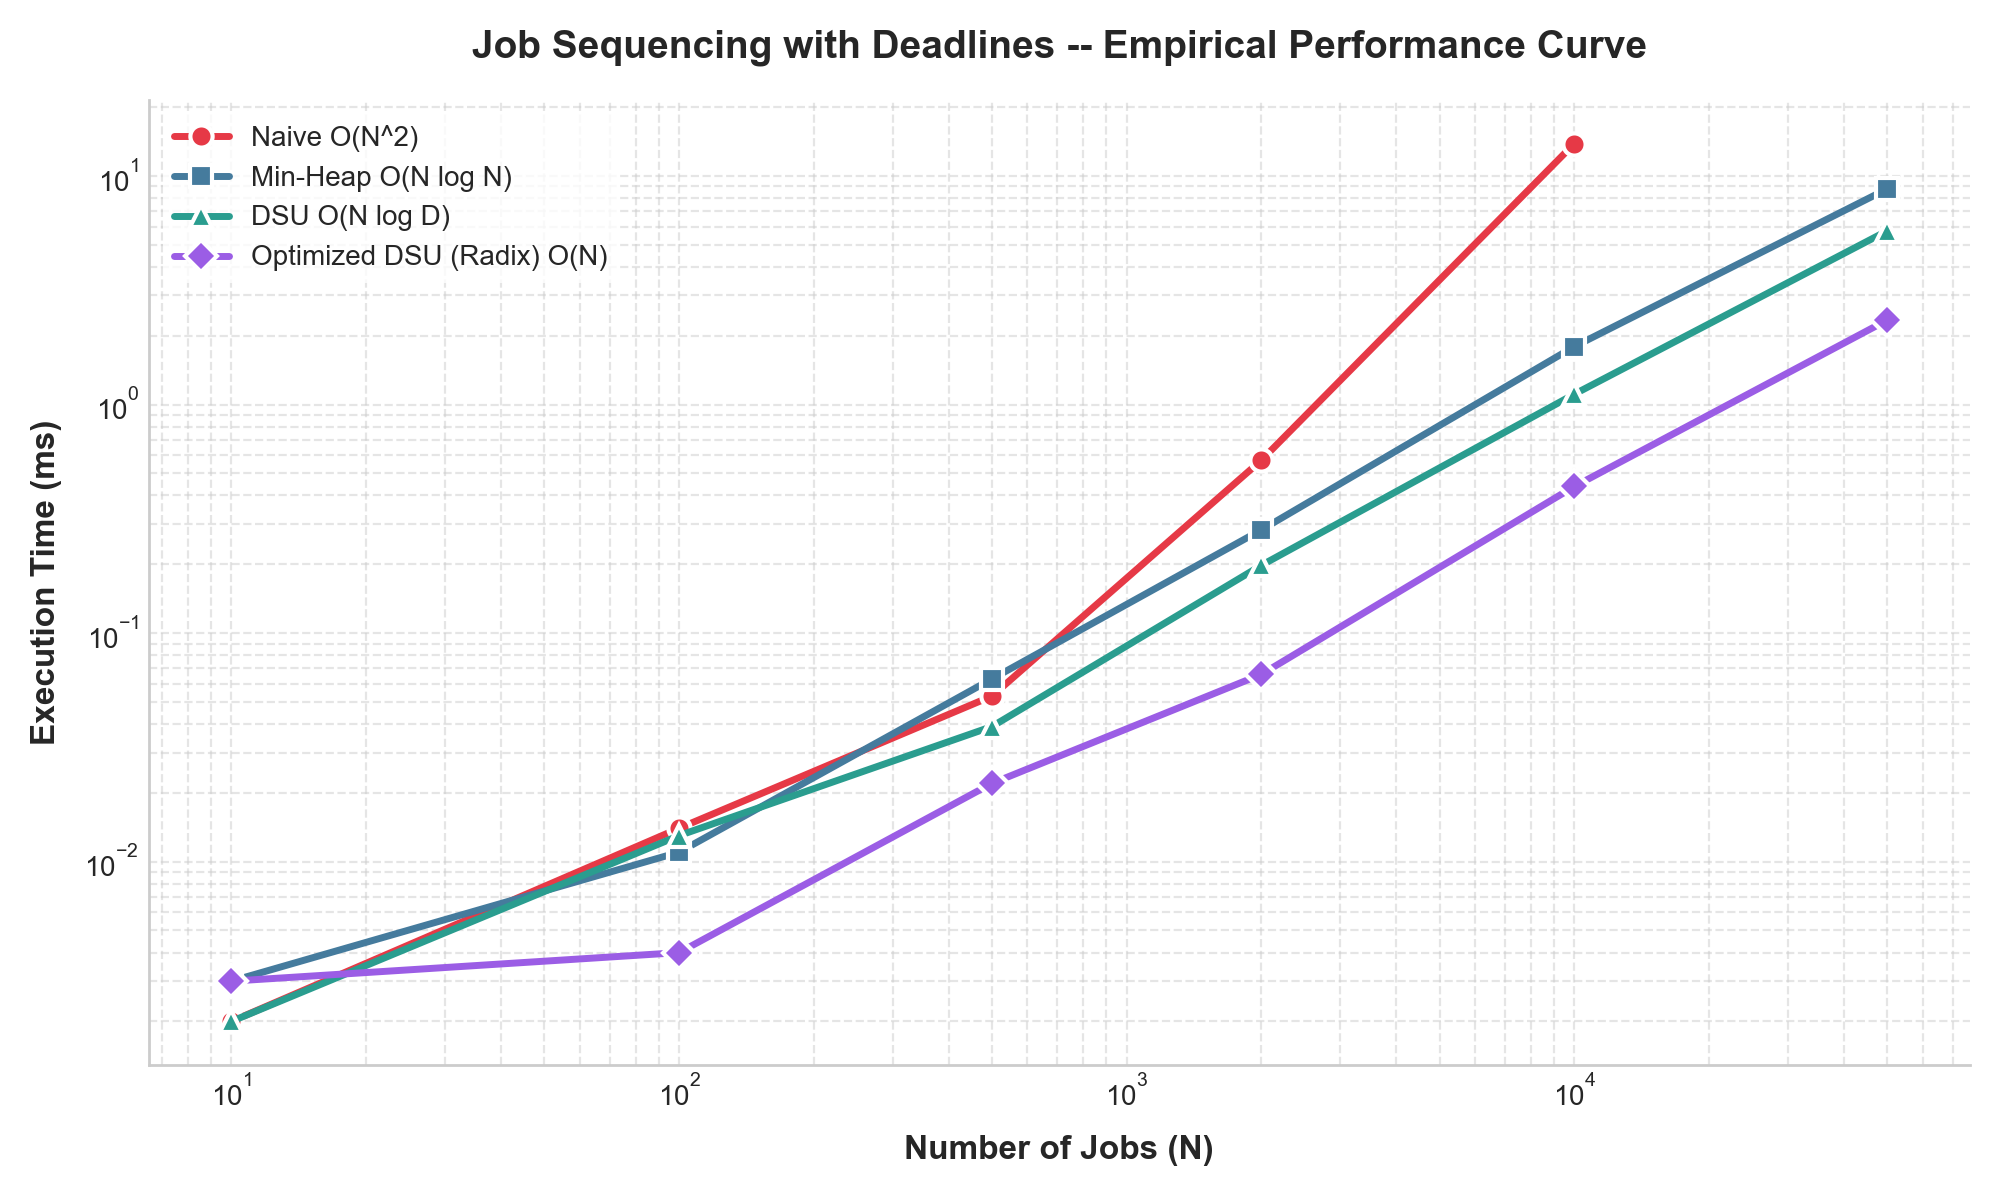
\includegraphics[width=0.85\textwidth]{job_sequencing_comparison.png}
\caption{Empirical execution times of the four algorithms on a log-log scale.}
\label{fig:comparison}
\end{figure}

The Naive algorithm shows quadratic growth, making it unusable at $N = 50,000$. Our proposed Radix-DSU algorithm is the fastest, executing in only 2.34 ms at $N = 50,000$ (over 2.5x faster than standard DSU and 4x faster than the Heap approach), demonstrating the value of eliminating the comparison sorting bottleneck.

\section{Real-World Industrial Applications and Extensions}

\subsection{Connection to Johnson's Algorithm (2-Machine Flow Shop)}
While single-machine job sequencing focuses on deadline constraints and profit maximization, real-world shop floors often require sequencing jobs across multiple machines in series. The classic 2-machine flow shop problem ($M_1 \to M_2$) is solved by \textbf{Johnson's Algorithm} in $O(N \log N)$ time.
Johnson's rule minimizes the total completion time (\textbf{makespan}) by sorting jobs into two groups: Group 1 ($t_{1i} < t_{2i}$) sorted in ascending order of processing time on $M_1$, and Group 2 ($t_{1i} \ge t_{2i}$) sorted in descending order of processing time on $M_2$. Group 1 is processed first, followed by Group 2.
In real-world settings, scheduling becomes much more difficult: when machines are subject to unavailability windows (e.g. maintenance), the makespan minimization problem becomes NP-hard (Rapine et al., 2013).

\subsection{Explainable AI (xAI) in Industrial Scheduling}
In real factory operations, automated schedules generated by optimization algorithms are frequently overridden or rejected by human floor operators. This is because these schedules act as "black-boxes" with no explanations for why a high-priority job was scheduled late.
To solve this, we propose integrating \textbf{Explainable AI (xAI)} with scheduling algorithms:
\begin{itemize}
    \item \textbf{Feature Attribution:} Using techniques like SHAP or LIME to attribute a job's position in the schedule to its profit, deadline, or machine processing time.
    \item \textbf{Counterfactual Explanations:} Providing actionable feedback to human managers: \textit{"If Job B's profit increases by 10\% or its deadline is extended by 1 hour, it will be scheduled today instead of next week."}
\end{itemize}
This combination of algorithmic efficiency and semantic explainability bridges the gap between theoretical algorithms and real-world operations.

\section{Conclusion}
In this report, we analyzed the Job Sequencing with Deadlines problem from both theoretical and empirical standpoints. We demonstrated that greedy scheduling is mathematically sound under Matroid Theory. Empirically, our proposed Radix-DSU algorithm reduces execution time significantly, achieving practically linear performance. Lastly, we connected this single-machine model to multi-machine environments via Johnson's algorithm and discussed how explainability (xAI) can increase human trust in automated industrial scheduling.

\end{document}
